\begin{itemize}
    \item In der Regel ist zumindest ein kurzes Theoriekapitel notwendig. Es nimmt Bezug auf das thematische Oberthema, aber natürlich nicht auf allgemeine theoretische Grundlagen etwa aus der Naturwissenschaft.
\end{itemize}

\section{Formula SAE Competitions}
The main idea of a Formula SAE competition is to conceive, design, fabricate, develop and compete with small, formula style, race cars.
The competition is split into two classes: Internal Combustion Engine Vehicle (\acrshort{cv}) and Electric Vehicle (\acrshort{ev}).
Additionally, a team can opt-in to take part in the Driverless Cup (\acrshort{dc}).
After a series of technical inspections in regards for safety and rules compliance, the vehicles will then compete in a series of static and dynamic events. In the end, the team with the most overall points will win the competition for its class or the \acrlong{dc}, respectively.

\subsection{Static Events}
The following static events are held: Business Plan Presentation, Cost and Manufacturing, and Engineering Design. In these events, the engineers have to present their car and their development processes to a panel of judges.

\begin{itemize}
    \item \textbf{Business Plan Presentation:} The team's ability to develop and deliver a comprehensive business model will be evaluated. The presentation should demonstrate how their self-developed race car could become a profitable business idea.
    \item \textbf{Cost and Manufacturing:} The financial planning of the car, including the manufacturing processes and costs associated with the construction of the race car are evaluated.
    \item \textbf{Engineering Design:} Evaluation of the engineering process and effort that went into the design of the vehicle. Technical aspects, the construction and key attributes of the car will be judged.
\end{itemize}

\subsection{Dynamic Events}
The following dynamic events are held: Skid Pad, Acceleration, Autocross, Endurance and Efficiency, and Trackdrive.
The dynamic events reveal the driving performance of the prototypes. Every discipline puts different abilities of the cars to the test.
\begin{itemize}
    \item \textbf{Skid Pad:} The skid pad track consists of two pairs of concentric circles in the shape of an eight. This track will test the lateral grip of the car.
    \begin{figure}[H]
        \centering
        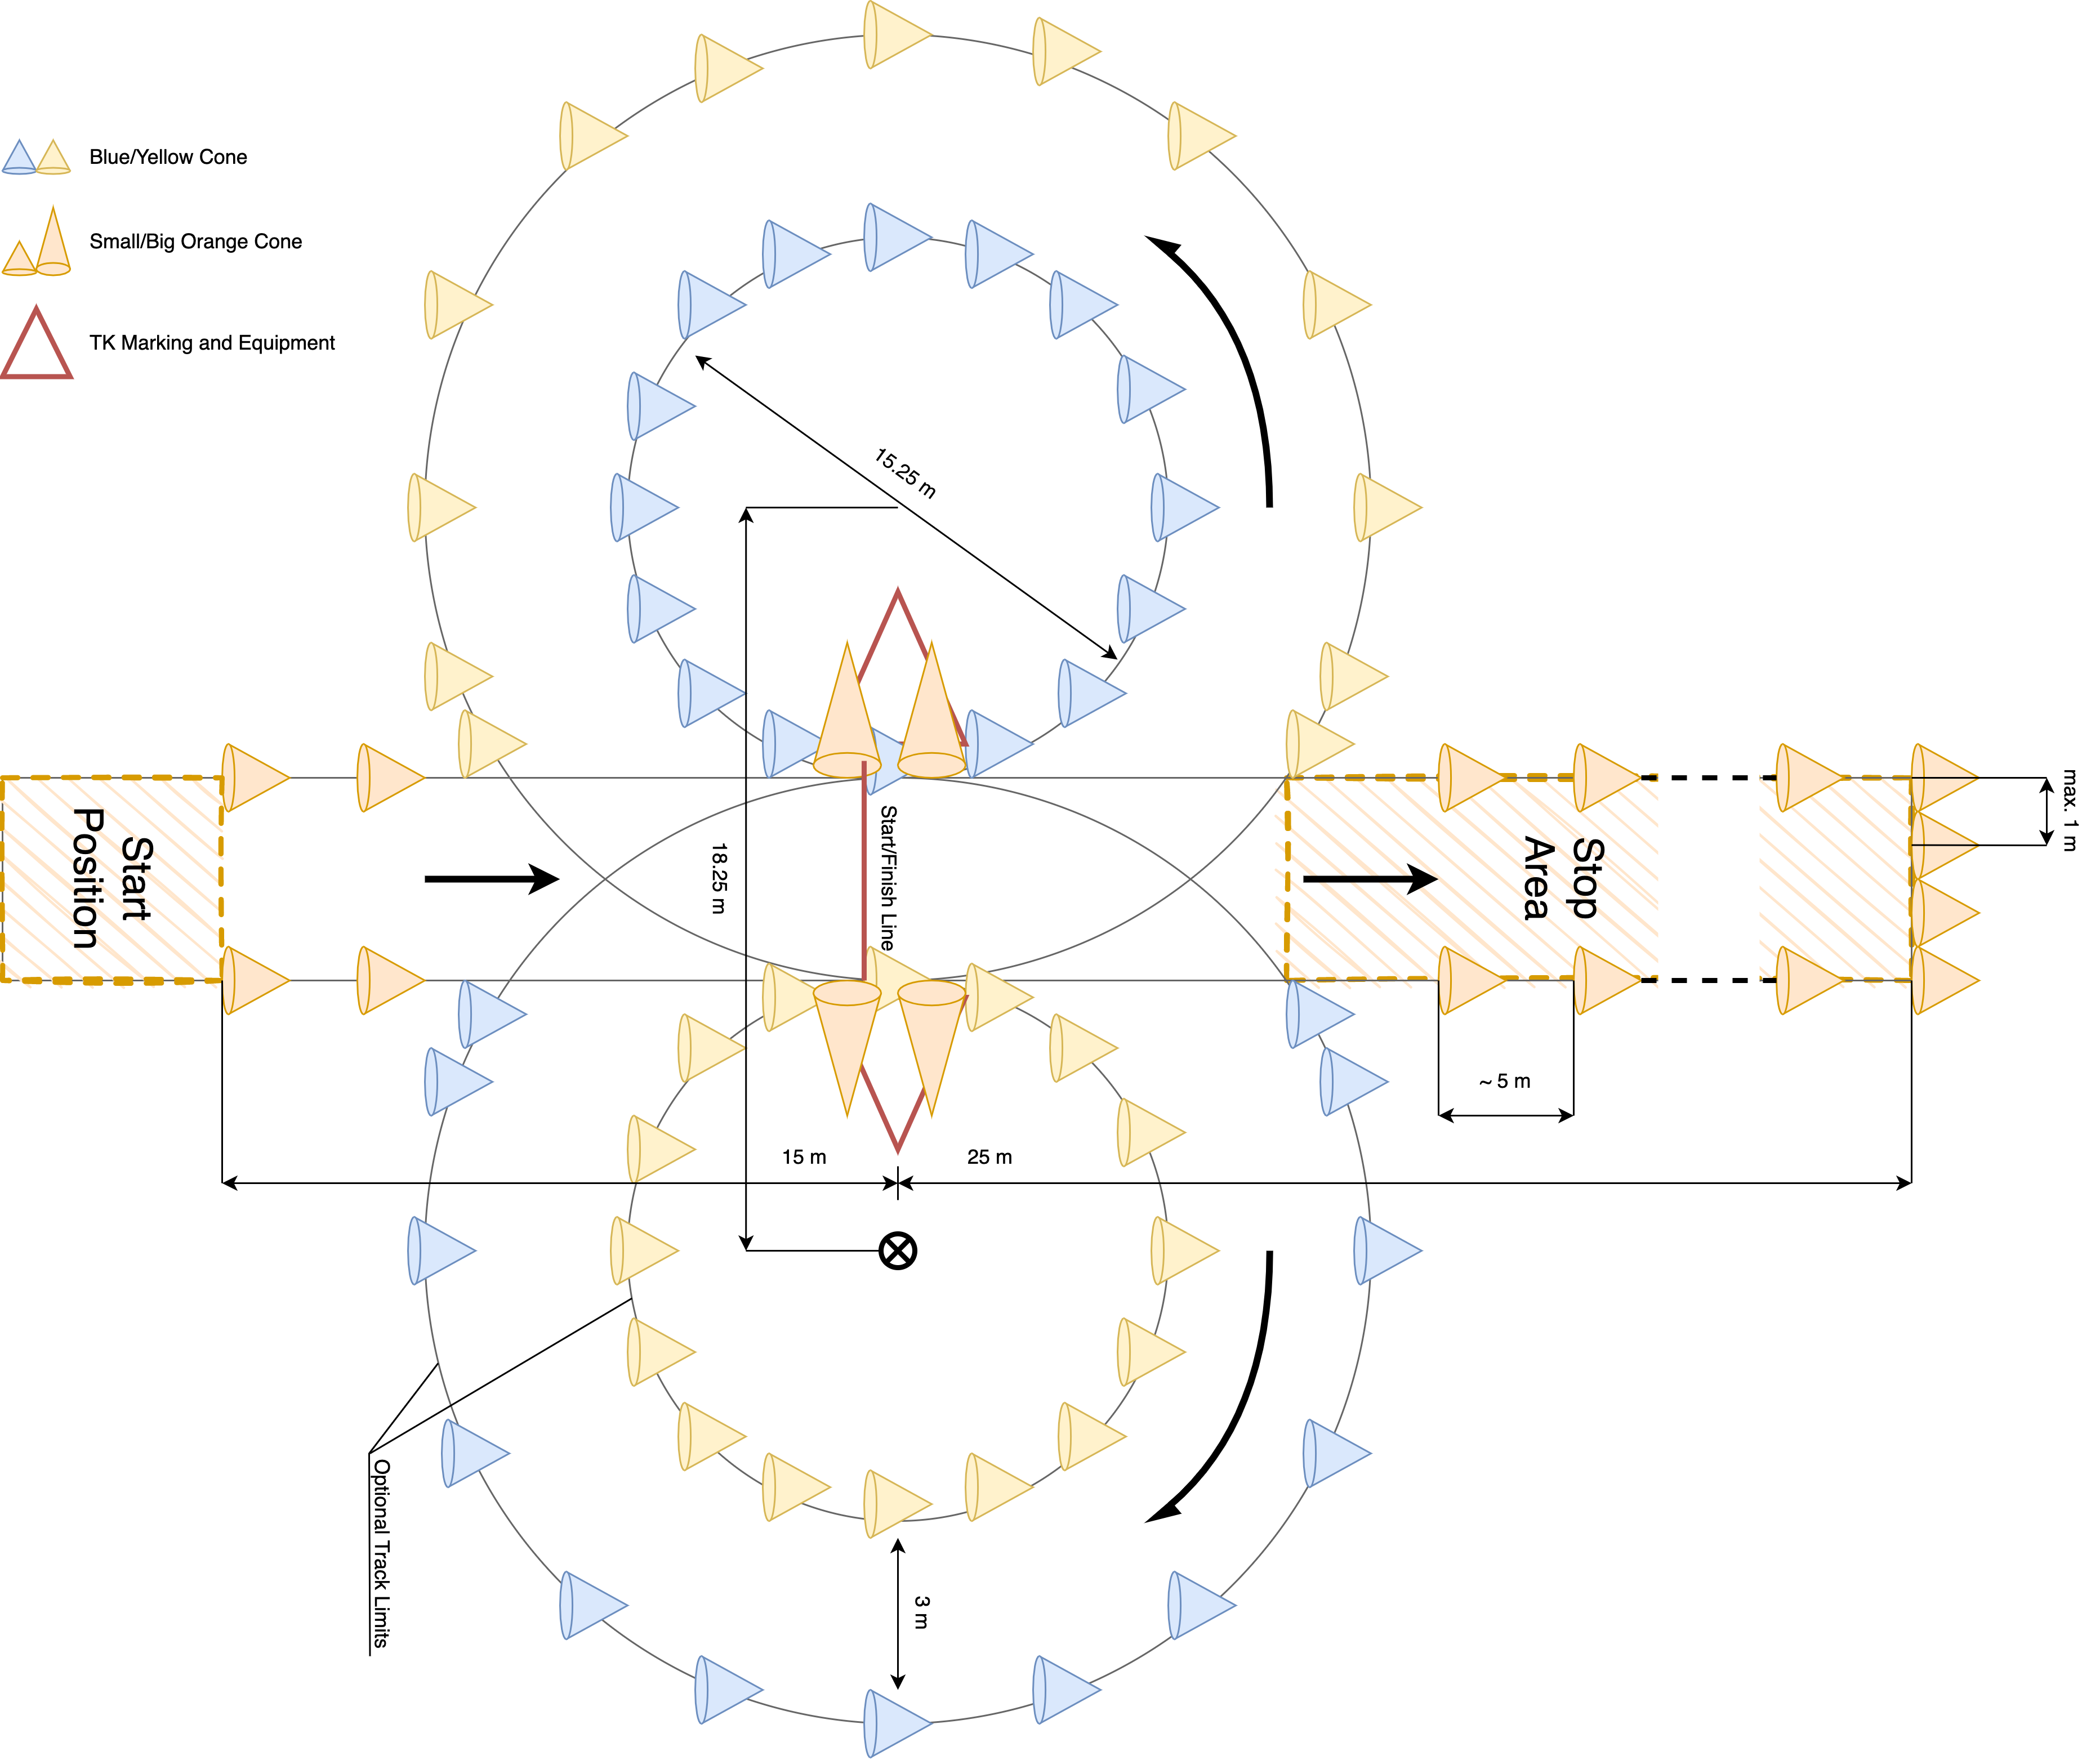
\includegraphics[width=\columnwidth]{FS_Event_Skid_Pad.png}
        \caption{Skid Pad track layout according to section D4 in the Formula Student Rules 2022 handbook \ref{fs_rules_2022_handbook}.}
        \label{fig:FS Skid Pad layout}
    \end{figure}
    \item \textbf{Acceleration:} An acceleration race over 75 m distance with a standing start, which tests the car acceleration in a straight line.
    \begin{figure}[H]
        \centering
        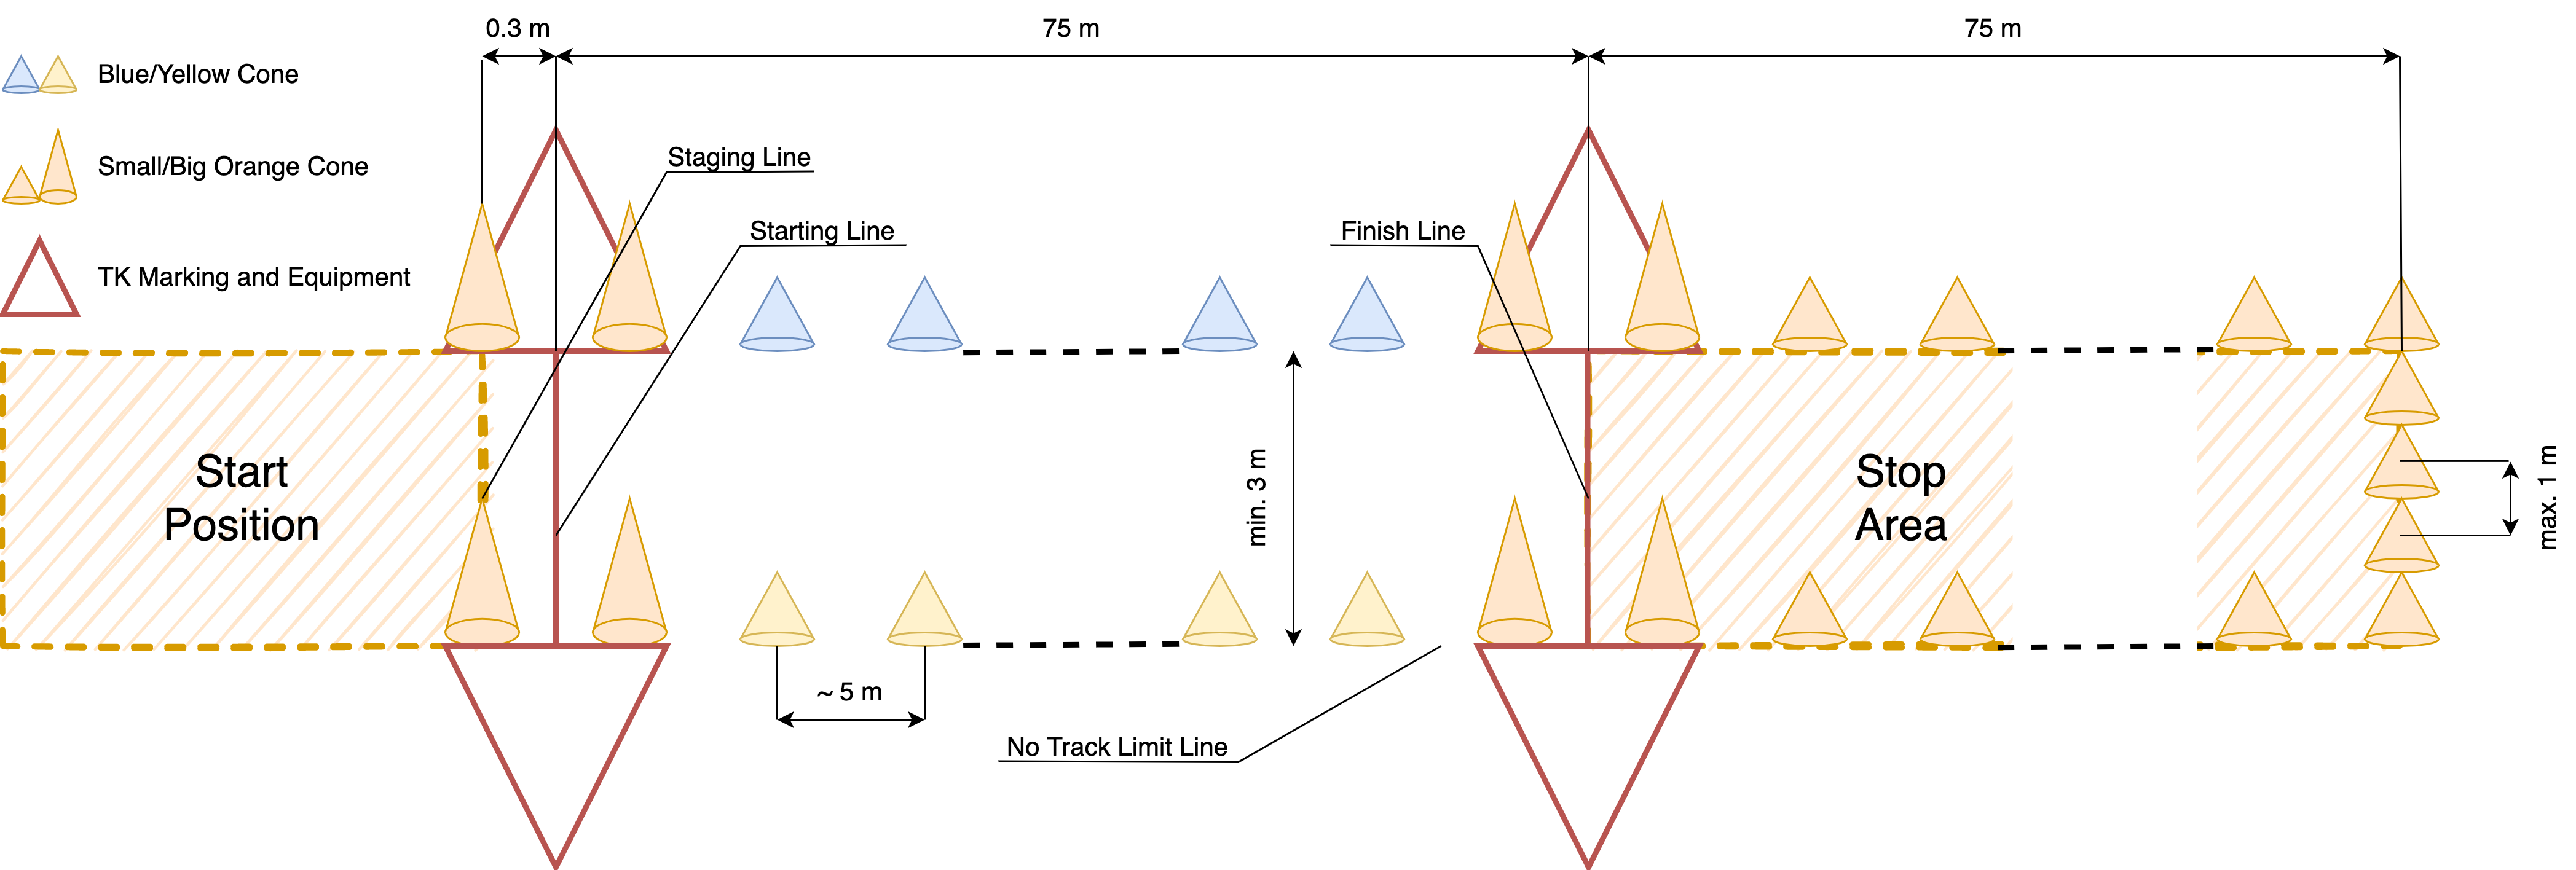
\includegraphics[width=\columnwidth]{FS_Event_Acceleration.png}
        \caption{Acceleration track layout according to section D5 in the Formula Student Rules 2022 handbook \ref{fs_rules_2022_handbook}.}
        \label{fig:FS Acceleration layout}
    \end{figure}
    \item \textbf{Autocross:} The autocross event tests the cars dynamic ability in a one lap sprint. The objective of the autocross event is to evaluate the car's manoeuvrability and handling qualities.
    \item \textbf{Endurance and Efficiency:} An endurance race over a distance of 22 km, including one driver change. One lap of the endurance track is approximately 1 km. The Efficiency scoring rates the consumed amount of energy in relation to the total time.
    \item \textbf{Trackdrive (DC Only):}  Over a distance of 10 rounds, the car has to prove its durability without a driver under long-term conditions.
    \begin{figure}[H]
        \centering
        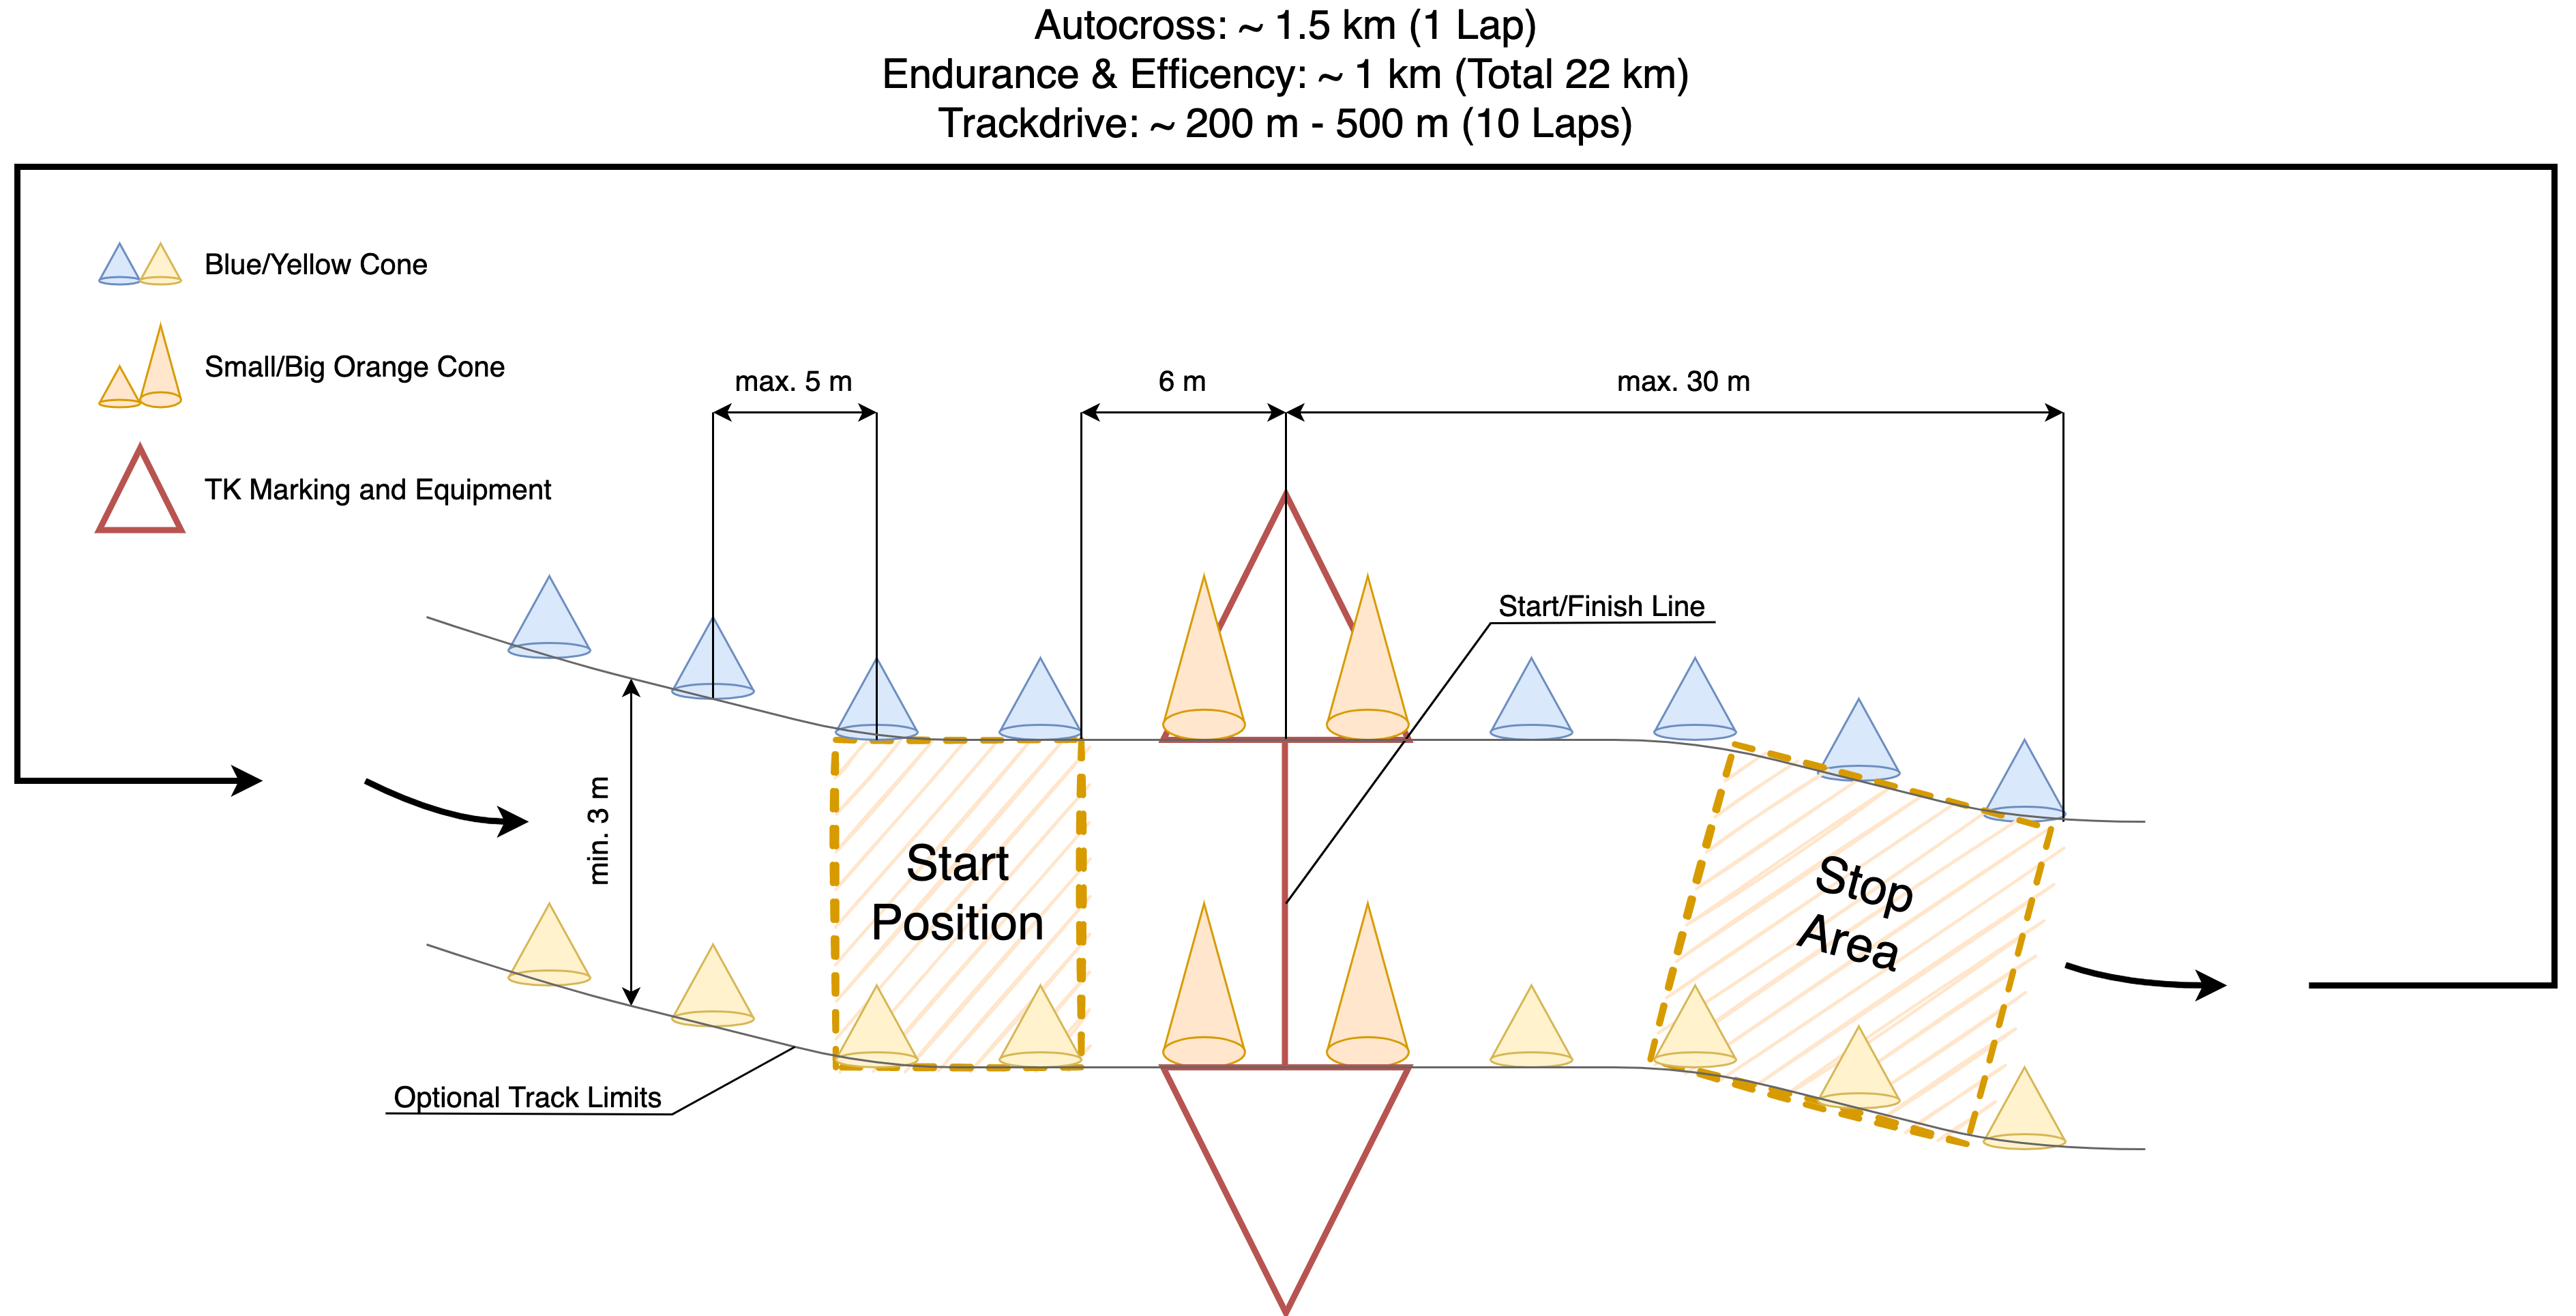
\includegraphics[width=\columnwidth]{FS_Event_Trackdrive.png}
        \caption{Base layout for the Autocross, Endurance and Trackdrive events according to sections D6, D7 and D8 in the Formula Student Rules 2022 handbook \ref{fs_rules_2022_handbook}.}
        \label{fig:FS Autocross, Endurance and Trackdrive layout}
    \end{figure}
\end{itemize}

\section{FSZHAW Autonomous System}
\begin{figure}[H]
    \centering
    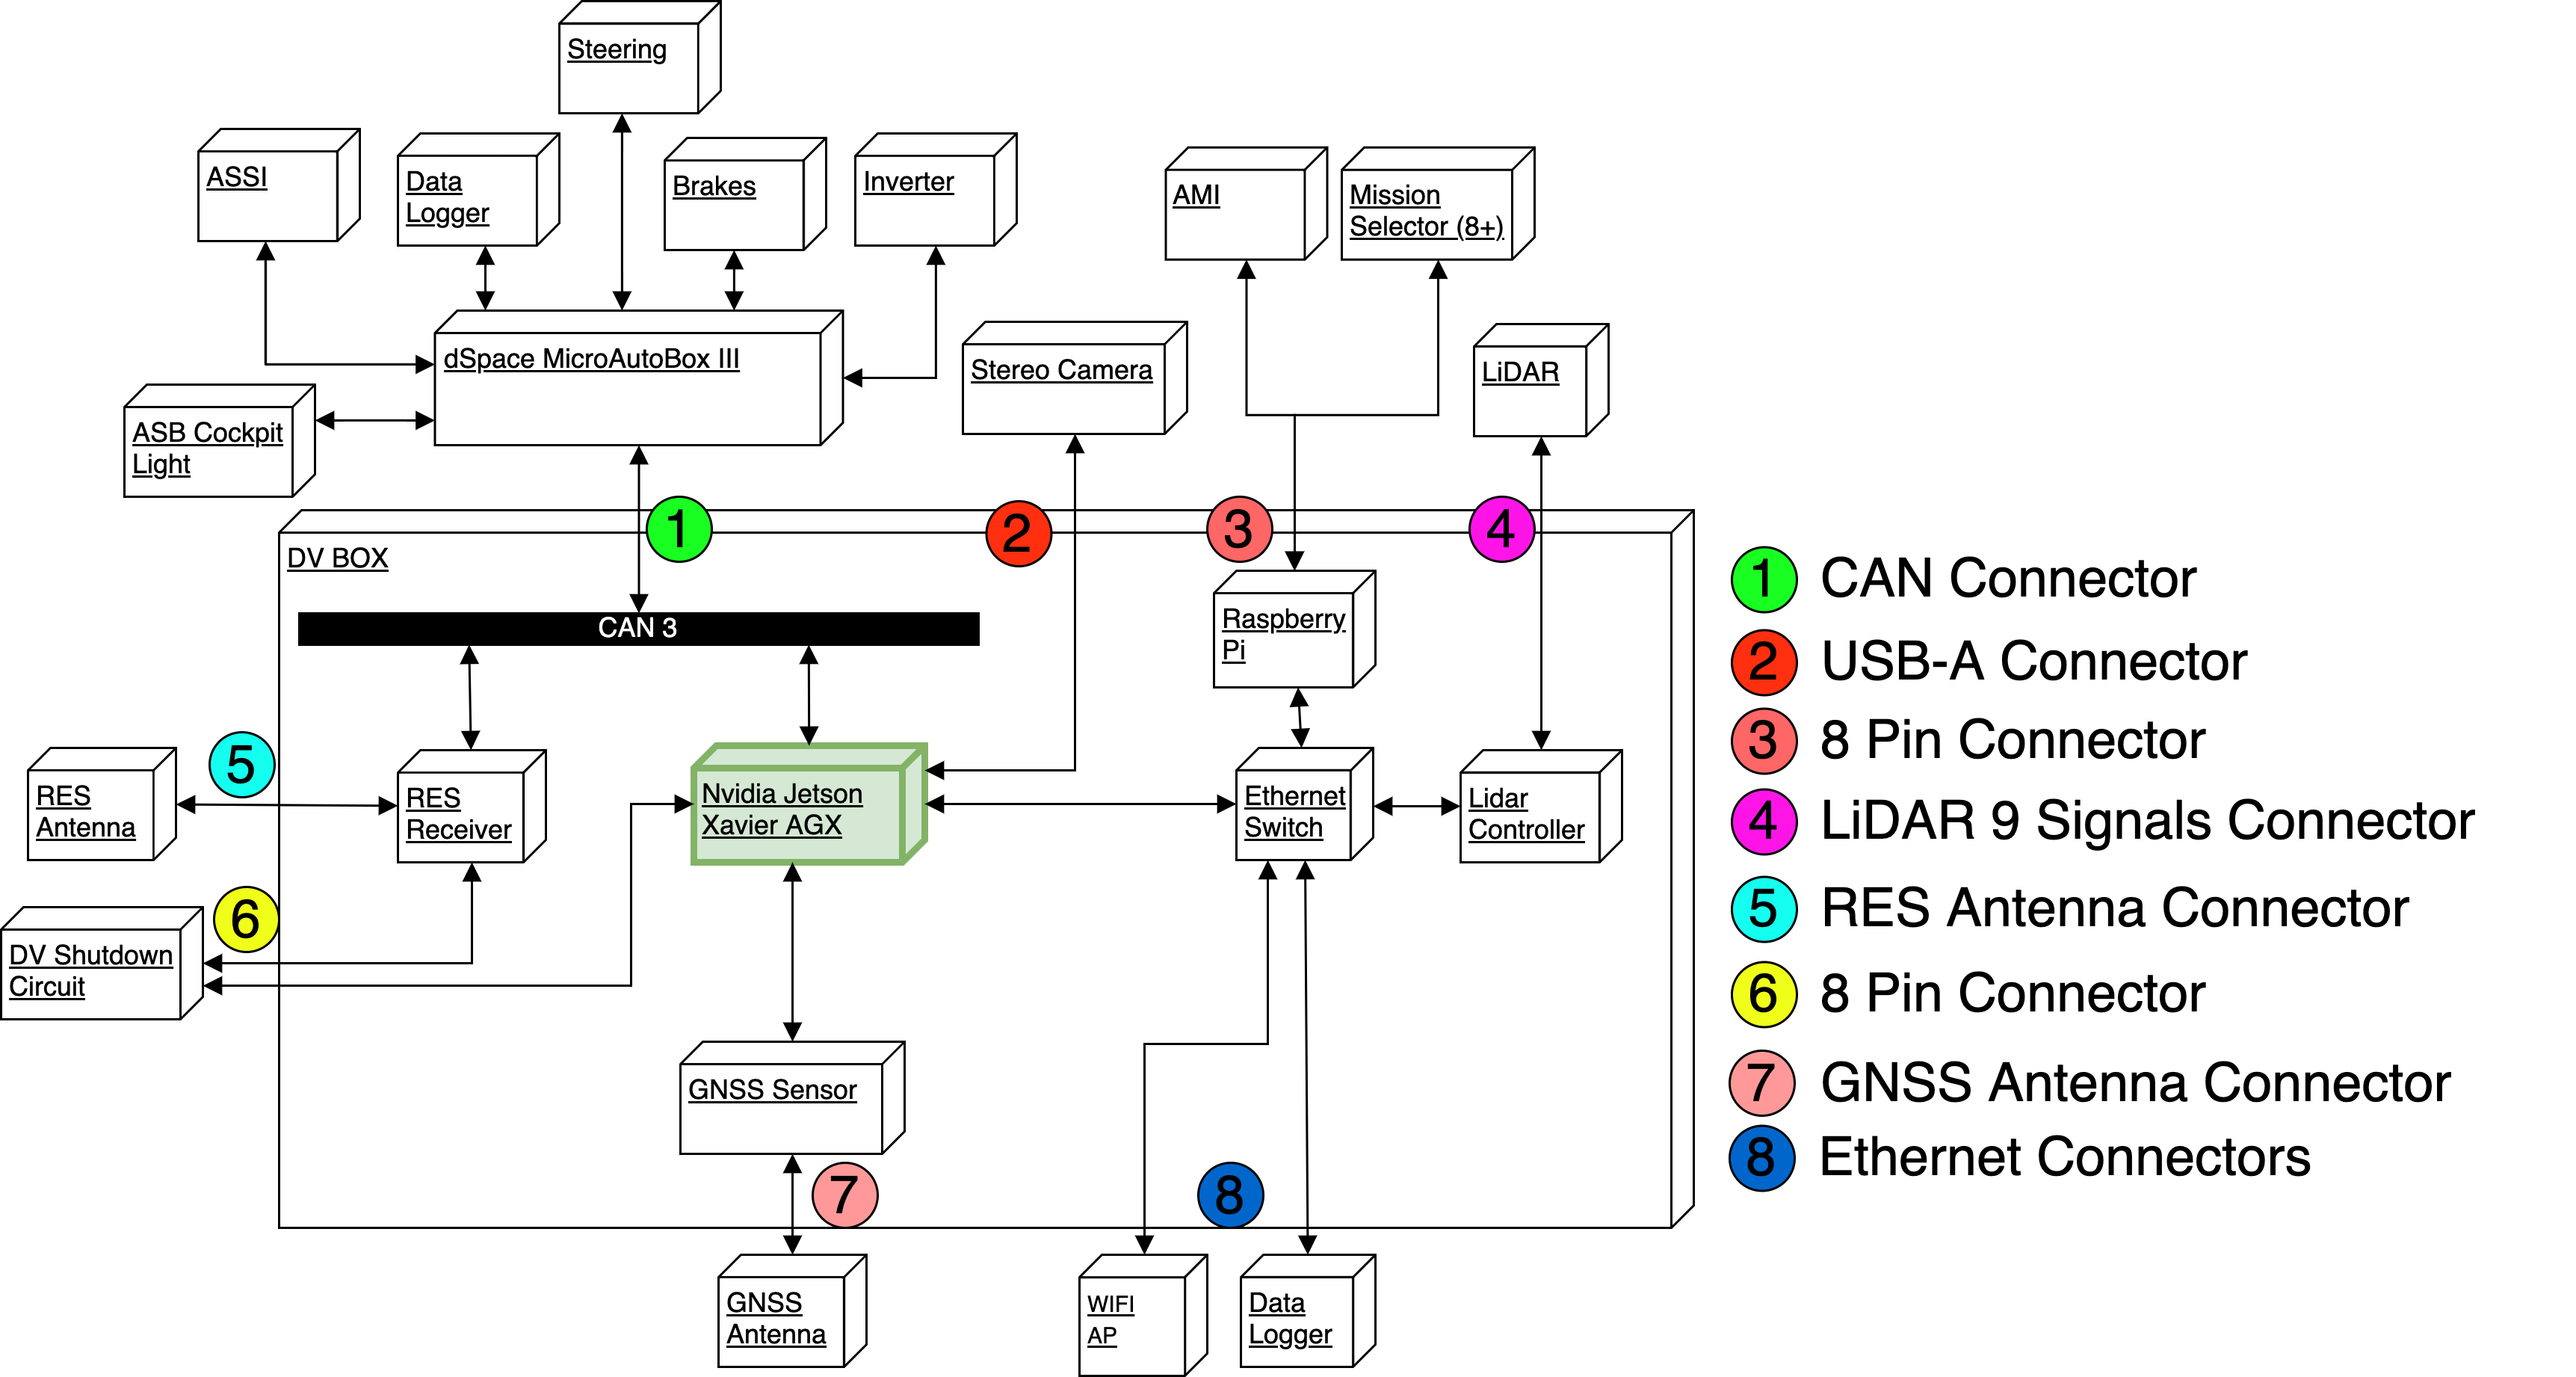
\includegraphics[width=\columnwidth]{AS_DV_Box.png}
    \caption{Autonomous System DV Box}
    \label{fig:AS DV Box}
\end{figure}

\begin{figure}[H]
    \centering
    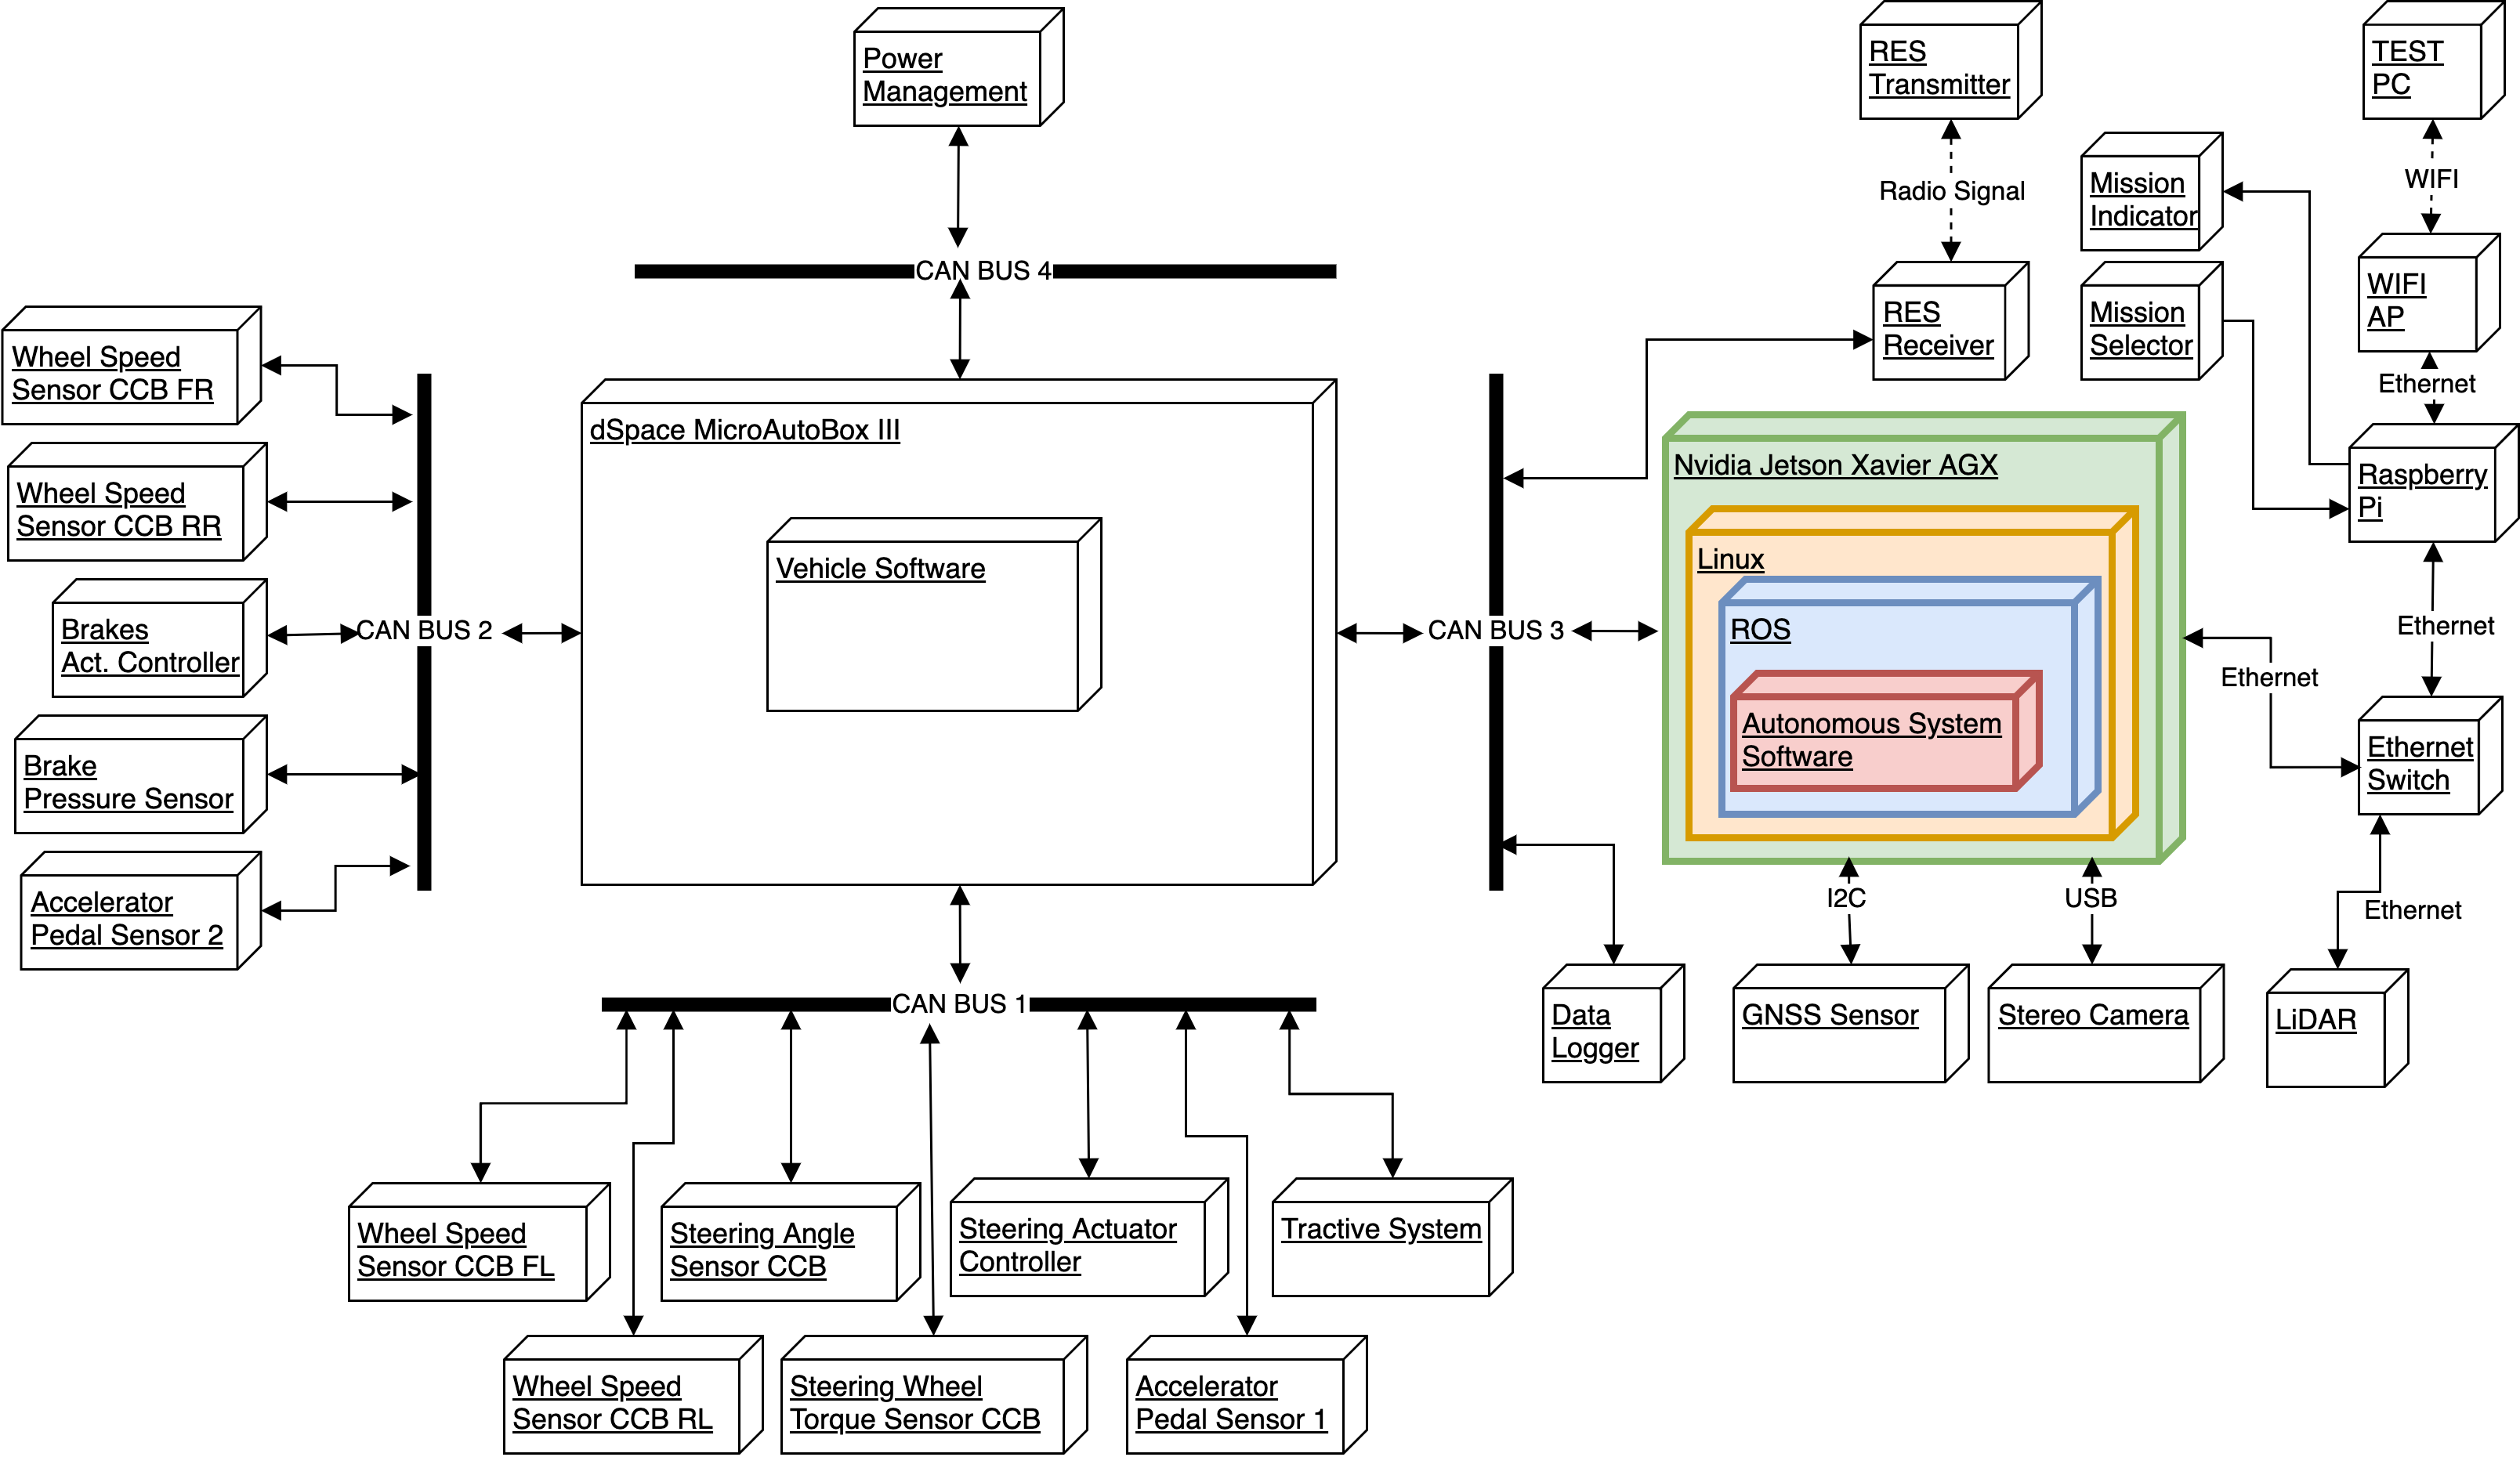
\includegraphics[width=\columnwidth]{AS_Deployment_Diagram.png}
    \caption{Autonomous System Deployment Diagram}
    \label{fig:AS Deployment Diagram}
\end{figure}

\begin{figure}[H]
    \centering
    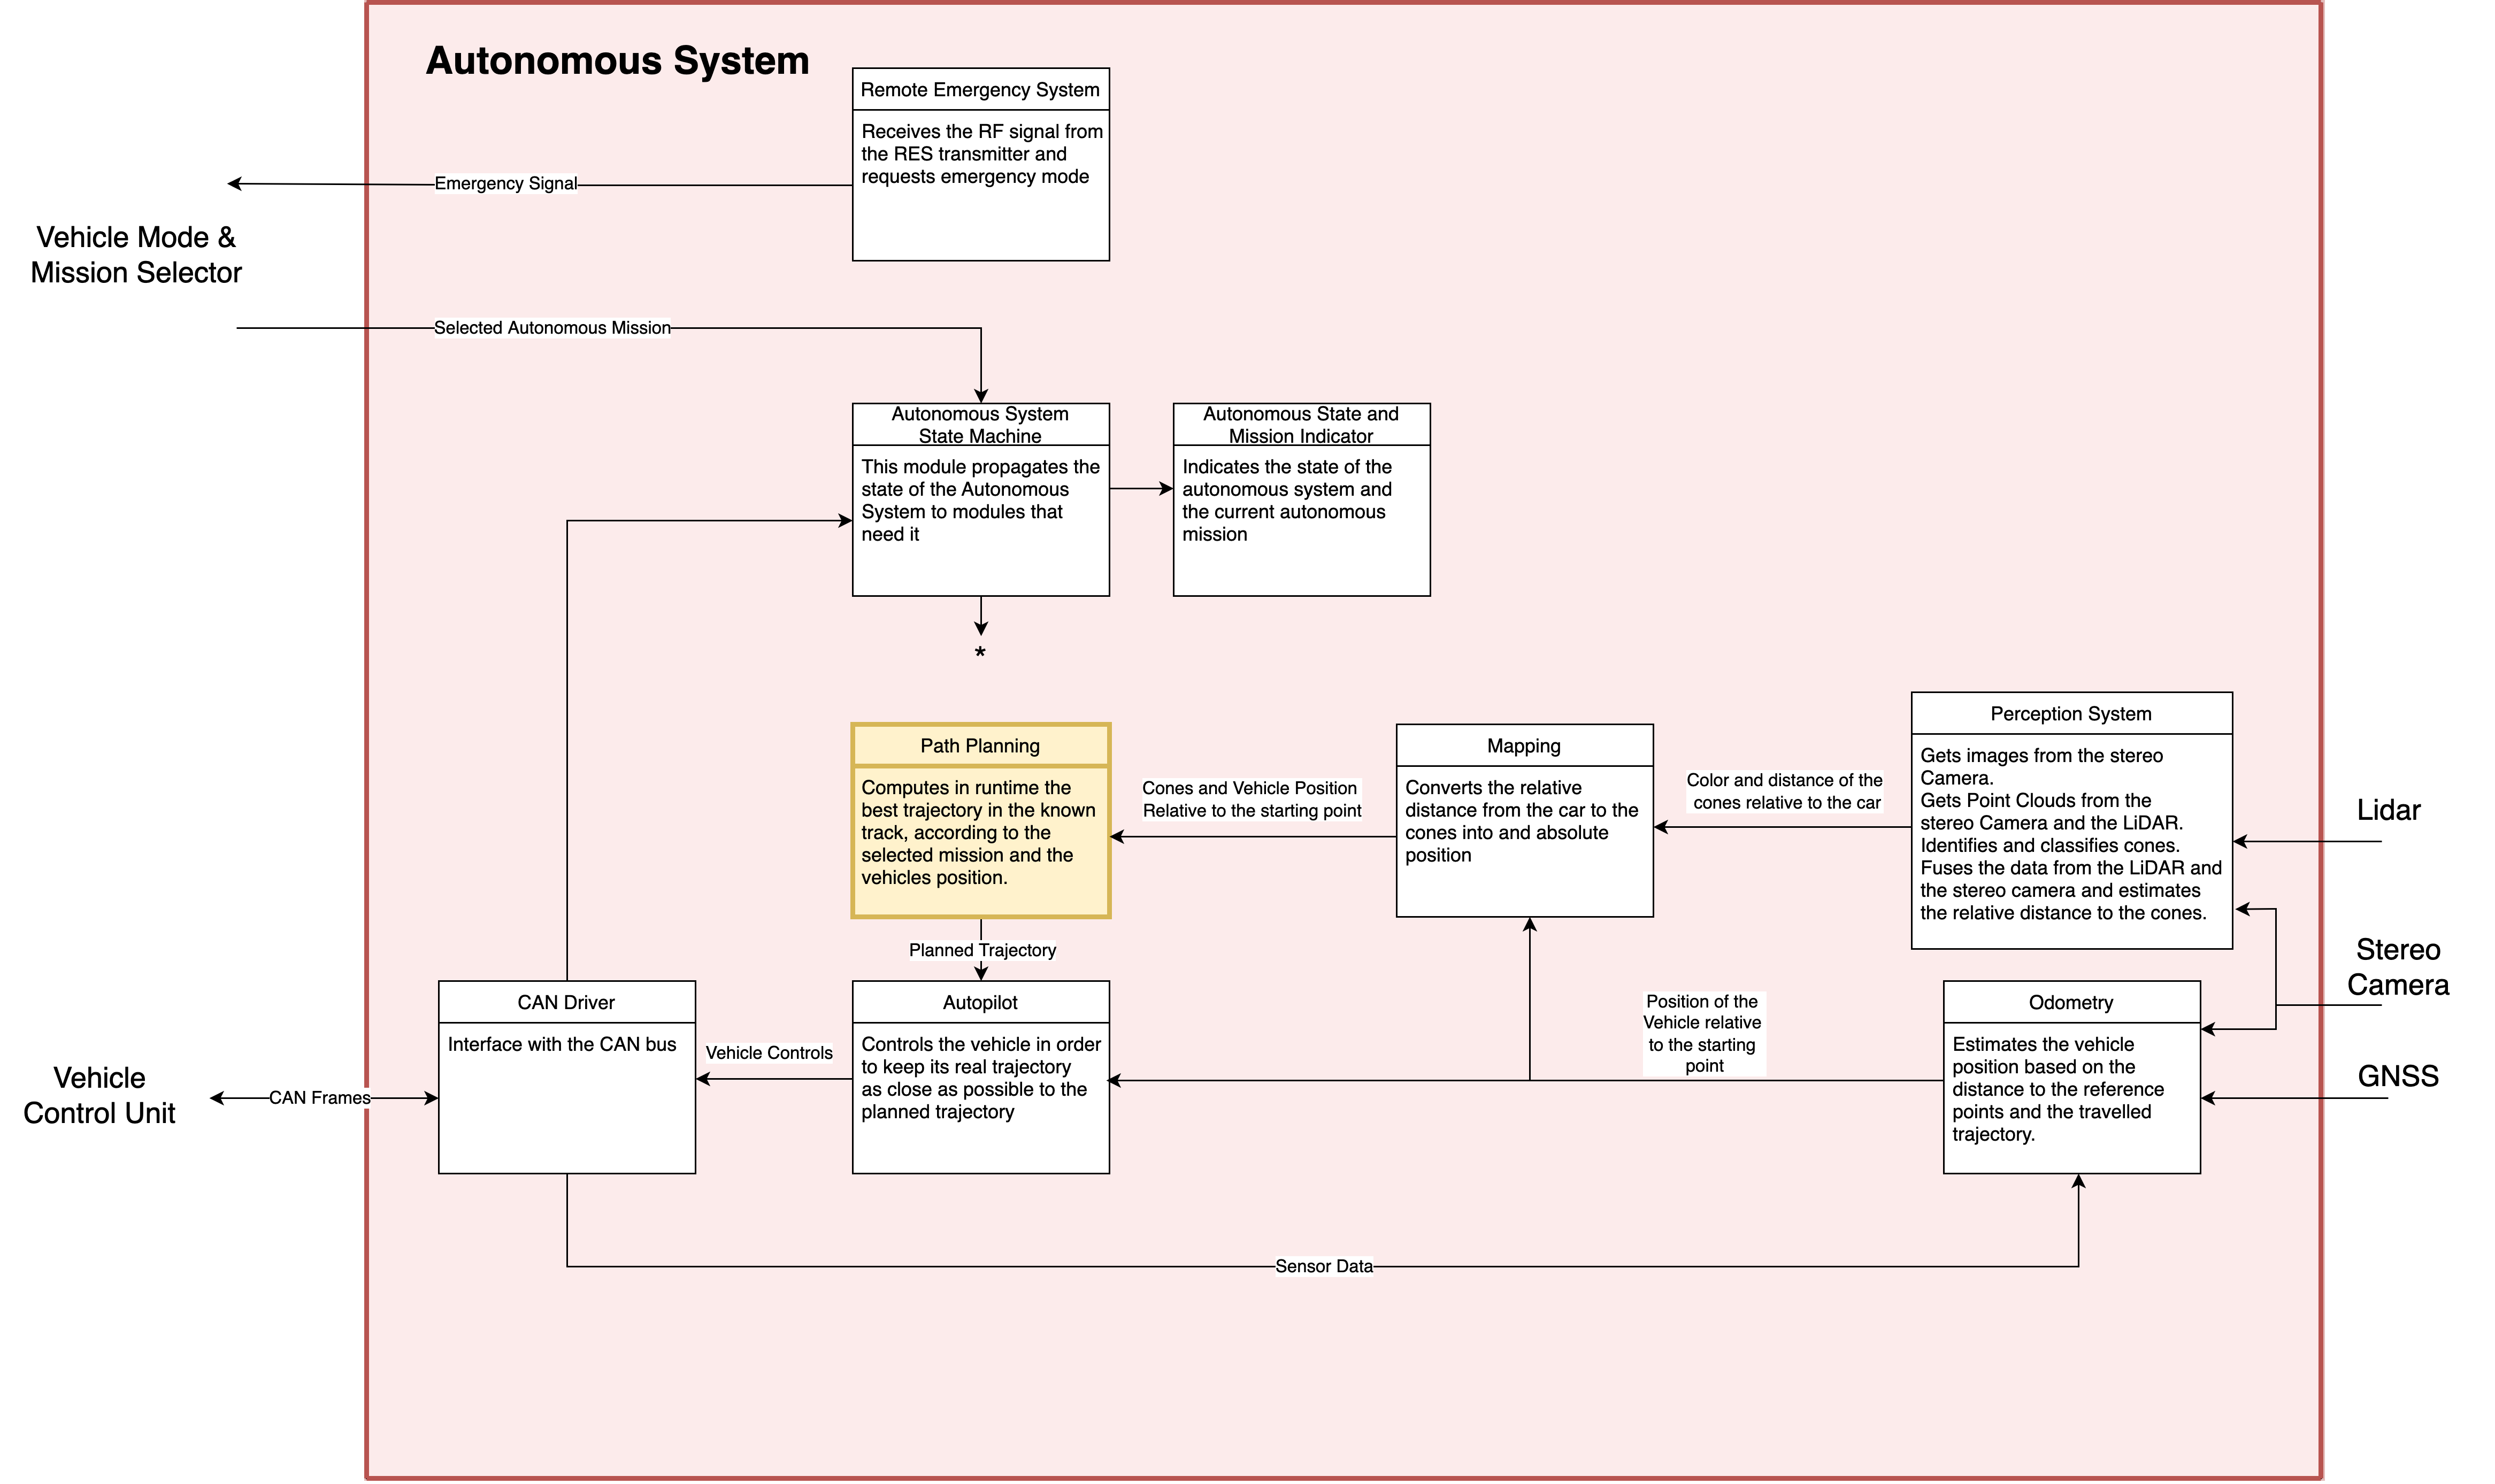
\includegraphics[width=\columnwidth]{AS_Component_Diagram.png}
    \caption{Autonomous System Component Diagram}
    \label{fig:AS Component Diagram}
\end{figure}

\section{Robot Operating System (ROS)}
The Robot Operating System (ROS) is not, like the name may suggest, a full-fledged operating system, but a set of software libraries and tools for the development of robot applications. The open-source robotics middleware comes shipped with capable developer tools, drivers and advanced algorithms. \cite{ros2_documentation}

There are currently two major versions of ROS which are seeing releases, ROS 1 and ROS 2. \cite{ros2_distributions} Beginning with releases after 'Foxy Fitzroy', releases in odd years will be non-LTS (Long Term Support) and will only be supported for 1.5 years, while new releases in even years are going to be long-term supported and will be supported for 5 years. \cite{ros2_releases_and_target_platforms}

The work done in this thesis have been done using the ROS 2 release 'Foxy Fitzroy', released on June 5th, 2020. This release will be supported till the end of May 2023. \cite{ros2_distributions}

\subsection{ROS Graph}
There are 5 main concepts of ROS 2 that make up the ROS (2) graph:
\begin{enumerate}
    \item Nodes
    \item Topics
    \item Services
    \item Parameters
    \item Actions
\end{enumerate}

The ROS graph is a network of ROS 2 elements which processes data simultaneously. The graph encompasses all executables and the connections between them.

\begin{figure}[H]
    \centering
    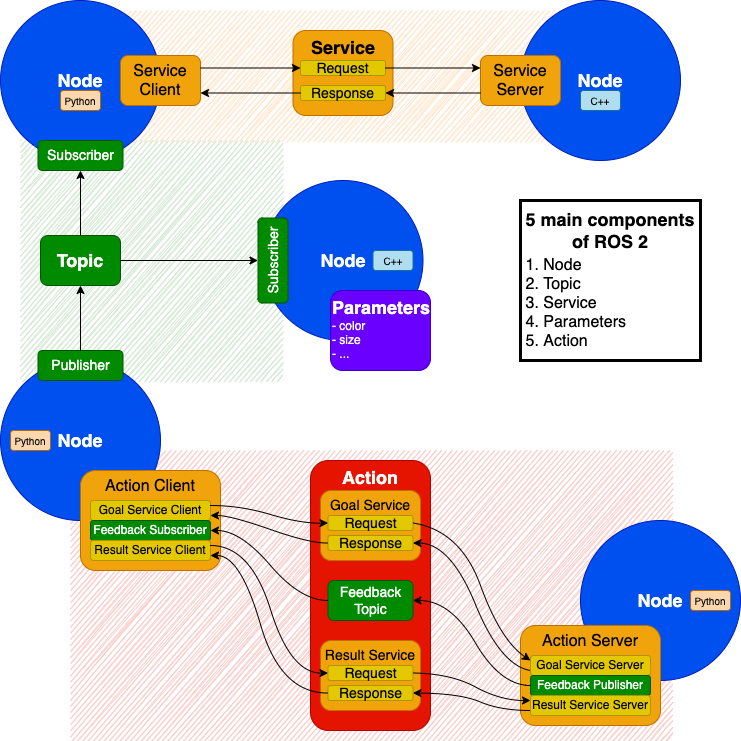
\includegraphics[width=\columnwidth]{ROS2_Main_Concepts.png}
    \caption{The five main concepts of ROS 2 pictured as a network of nodes.}
    \label{fig:ROS 2 main concepts}
\end{figure}

\subsubsection{Nodes}
A node is a fundamental ROS 2 element that serves a single, modular purpose in a robotics system. % https://docs.ros.org/en/foxy/Tutorials/Understanding-ROS2-Nodes.html

\subsubsection{Topics}
 Nodes publish information over topics, which allows any number of other nodes to subscribe to and access that information. % https://docs.ros.org/en/foxy/Tutorials/Topics/Understanding-ROS2-Topics.html

\subsubsection{Services}
Services are based on a call-and-response model, versus topics’ publisher-subscriber model. Services only provide data when they are specifically called by a client. % https://docs.ros.org/en/foxy/Tutorials/Services/Understanding-ROS2-Services.html

\subsubsection{Parameters}
Nodes have parameters to define their default configuration values. %https://docs.ros.org/en/foxy/Tutorials/Parameters/Understanding-ROS2-Parameters.html

\subsubsection{Actions}
Actions are built on topics and services and consist of a goal, feedback, and a result. Actions are like services that allow you to execute long-running tasks, provide regular feedback, and are cancellable. % https://docs.ros.org/en/foxy/Tutorials/Understanding-ROS2-Actions.html

\section{Driverless}
\lipsum[1]

\section{Path Planning Algorithms}
Path planning algorithms are used in many environments for example in assembling a car with a robot arm, parking a car autonomously or finding a landmine with a robot in a military operation. 

\subsection{Overview}
A path can be if a human goes from A to B and follows certain signs for example when hiking on a mountain. Otherwise, a human can follow a path that is generated on a GPS system in a car. The difference lies by a manual plan versus a generated plan by a machine. This section addresses only the generated one.

The planning consists of a state, time that is needed, actions, initial / goal state, criterion and a plan. The state is normally represented by a planning algorithm. Time is based on a sequence of decision that has to be made in a certain time. Actions manipulate the state and cover how the state should be changed. The initial and goal state defines where the planner should start and finish.
The criterion defines the outcome and the boundaries of the planner. The type of the criterion is either based on the feasibility or optimality. Feasibility covers the arrival of the goal state without the concern of efficiency. Optimality finds a plan with an optimized performance in mind. The plan in general covers the strategy or behaviour on a decision maker.
\cite{planning_algorithms_steven_m_lavalle}

\subsection{Algorithms, Planners and Plans}
An algorithm usually consists of a machine and environment where there are actuations from the machine to the environment and sensing from the environment to the machine. The problem in planning is often that the machine interacts with the physical world which has uncountable different influences on the plan that has to be calculated. This is why the environment is often an approximation of the real world since not every sensing mechanism from the environment to the machine can be processed.

Planners are constructing plans. They are either a machine or a human. When the planner is a machine then it is usually a planning algorithm. If the planner is a human then the human itself is the algorithm which makes the decision.

The plans can be used in three different ways: Execution, refinement or hierarchical inclusion. Execution runs the plan on a simulation or a robot which is connected to the real world. Refinement tries to find a better plan. The hierarchical inclusion gives the plan to a higher level plan that is consisting of sub plans.

\cite{planning_algorithms_steven_m_lavalle}

\subsection{Path Planning Algorithm Categories}
A path planning algorithm can be categorized in one of the following groups:
\begin{itemize}
    \item Motion Planning
    \item Decision-Theoretic Planning
    \item Planning under Differential Constraints
\end{itemize}

\subsubsection{Motion Planning}

Motion planning is interested in planning in continuous state spaces. This means that the space is not static and changes in relation to time. IT is also called motion planning or planning in continuous state spaces.

\textbf{Implicit Representation} of a state space in motion planning must be dealt with in planning algorithms. Implicit representations become more important in motion planning as the state space is uncountably infinite. It also tries to define 2D and 3D geometric models and transforms them. State spaces arise from these problems.

\textbf{Continuous $\rightarrow$ discrete} is the central theme in motion planning to transform models. Motion planning also covers combinatorial motion planning, which means with the input model the algorithm builds a representation of the original problem. There is also the field of sampling-based motion planning.

\textbf{Geometric Representation and Transformation} to start defining a motion planning algorithm. It defines a body of a system in a space and how it transforms for example moves. There are also chains of movements of a body.
\textbf{The Configuration Space} is needed for the motion planning algorithm to define the space in which is a set of possible transformations that could be applied to a robot.
\textbf{Sampling-Based Motion Planning} is a field in motion planning that covers sampling-based algorithms. Sampling-based planning algorithm uses a collision detection as a "black box" which is separated to geometric and kinematic models motion planning.
\textbf{Combinatorial Motion Planning} covers finding path in a continuous space without the restoration of approximations. 
\textbf{Extensions of Basic Motion Planning} defines flavours of motion planning algorithms. There are for example the time-varying problems which defined in the planning formulation.
\textbf{Feedback Motion Planning} describes a class of motion planning algorithms that are taking feedback for example from the real world into account.

\subsubsection{Decision-Theoretic Planning}
\textbf{Basic Decision Theory}
\textbf{Sequential Decision Theory}
\textbf{Sensors and Information Spaces}
\textbf{Planning Under Sensing Uncertainty}

\subsubsection{Planning under Differential Constraints}
\textbf{Differential Models}
\textbf{Sampling-Based Planning Under Differential Constraints}
\textbf{System Theory and Analytical Techniques}

\section{Hardware}

\subsection{Nvidia Jetson}
\lipsum[1]

\subsection{Lidar}
\lipsum[1]

\subsection{Stereo Camera}
\lipsum[1]

\section{Languages and Tools}

\begin{itemize}
    \item ROS 2
    \item Python
    \item LaTeX
    \item Git
    \item VS Code
    \item Azure DevOps
    \item GitHub
    \item Simulation tools
    \item other tools
\end{itemize}

\lipsum[1]